%%%%%%%%%%%%%%%%%%%%%%%%%%%%%%%%%%%%%%%%%
% Masters/Doctoral Thesis 
% LaTeX Template
% Version 2.5 (27/8/17)
%
% This template was downloaded from:
% http://www.LaTeXTemplates.com
%
% Version 2.x major modifications by:
% Vel (vel@latextemplates.com)
%
% This template is based on a template by:
% Steve Gunn (http://users.ecs.soton.ac.uk/srg/softwaretools/document/templates/)
% Sunil Patel (http://www.sunilpatel.co.uk/thesis-template/)
%
% Template license:
% CC BY-NC-SA 3.0 (http://creativecommons.org/licenses/by-nc-sa/3.0/)
%
%%%%%%%%%%%%%%%%%%%%%%%%%%%%%%%%%%%%%%%%%

%----------------------------------------------------------------------------------------
%	PACKAGES AND OTHER DOCUMENT CONFIGURATIONS
%----------------------------------------------------------------------------------------

\documentclass[
11pt, % The default document font size, options: 10pt, 11pt, 12pt
%oneside, % Two side (alternating margins) for binding by default, uncomment to switch to one side
english, % ngerman for German
singlespacing, % Single line spacing, alternatives: onehalfspacing or doublespacing
%draft, % Uncomment to enable draft mode (no pictures, no links, overfull hboxes indicated)
%nolistspacing, % If the document is onehalfspacing or doublespacing, uncomment this to set spacing in lists to single
%liststotoc, % Uncomment to add the list of figures/tables/etc to the table of contents
%toctotoc, % Uncomment to add the main table of contents to the table of contents
%parskip, % Uncomment to add space between paragraphs
%nohyperref, % Uncomment to not load the hyperref package
headsepline, % Uncomment to get a line under the header
%chapterinoneline, % Uncomment to place the chapter title next to the number on one line
%consistentlayout, % Uncomment to change the layout of the declaration, abstract and acknowledgements pages to match the default layout
]{MastersDoctoralThesis} % The class file specifying the document structure

\usepackage[utf8]{inputenc} % Required for inputting international characters
\usepackage[T1]{fontenc} % Output font encoding for international characters

\usepackage{mathpazo} % Use the Palatino font by default

\usepackage[backend=bibtex,style=authoryear,natbib=true]{biblatex} % Use the bibtex backend with the authoryear citation style (which resembles APA)

\addbibresource{example.bib} % The filename of the bibliography

\usepackage[autostyle=true]{csquotes} % Required to generate language-dependent quotes in the bibliography

%----------------------------------------------------------------------------------------
%	MARGIN SETTINGS
%----------------------------------------------------------------------------------------

\geometry{
	paper=a4paper, % Change to letterpaper for US letter
	inner=2.5cm, % Inner margin
	outer=3.8cm, % Outer margin
	bindingoffset=.5cm, % Binding offset
	top=1.5cm, % Top margin
	bottom=1.5cm, % Bottom margin
	%showframe, % Uncomment to show how the type block is set on the page
}

%----------------------------------------------------------------------------------------
%	THESIS INFORMATION
%----------------------------------------------------------------------------------------

\thesistitle{Thesis Title} % Your thesis title, this is used in the title and abstract, print it elsewhere with \ttitle
\supervisor{Dr. James \textsc{Smith}} % Your supervisor's name, this is used in the title page, print it elsewhere with \supname
\examiner{} % Your examiner's name, this is not currently used anywhere in the template, print it elsewhere with \examname
\degree{Doctor of Philosophy} % Your degree name, this is used in the title page and abstract, print it elsewhere with \degreename
\author{John \textsc{Smith}} % Your name, this is used in the title page and abstract, print it elsewhere with \authorname
\addresses{} % Your address, this is not currently used anywhere in the template, print it elsewhere with \addressname

\subject{Biological Sciences} % Your subject area, this is not currently used anywhere in the template, print it elsewhere with \subjectname
\keywords{} % Keywords for your thesis, this is not currently used anywhere in the template, print it elsewhere with \keywordnames
\university{\href{http://www.university.com}{University Name}} % Your university's name and URL, this is used in the title page and abstract, print it elsewhere with \univname
\department{\href{http://department.university.com}{Department or School Name}} % Your department's name and URL, this is used in the title page and abstract, print it elsewhere with \deptname
\group{\href{http://researchgroup.university.com}{Research Group Name}} % Your research group's name and URL, this is used in the title page, print it elsewhere with \groupname
\faculty{\href{http://faculty.university.com}{Faculty Name}} % Your faculty's name and URL, this is used in the title page and abstract, print it elsewhere with \facname

\AtBeginDocument{
\hypersetup{pdftitle=\ttitle} % Set the PDF's title to your title
\hypersetup{pdfauthor=\authorname} % Set the PDF's author to your name
\hypersetup{pdfkeywords=\keywordnames} % Set the PDF's keywords to your keywords
}

\begin{document}

\frontmatter % Use roman page numbering style (i, ii, iii, iv...) for the pre-content pages

\pagestyle{plain} % Default to the plain heading style until the thesis style is called for the body content

%----------------------------------------------------------------------------------------
%	TITLE PAGE
%----------------------------------------------------------------------------------------

\begin{titlepage}
\begin{center}

\vspace*{.06\textheight}
{\scshape\LARGE \univname\par}\vspace{1.5cm} % University name
\textsc{\Large Doctoral Thesis}\\[0.5cm] % Thesis type

\HRule \\[0.4cm] % Horizontal line
{\huge \bfseries \ttitle\par}\vspace{0.4cm} % Thesis title
\HRule \\[1.5cm] % Horizontal line
 
\begin{minipage}[t]{0.4\textwidth}
\begin{flushleft} \large
\emph{Author:}\\
\href{http://www.johnsmith.com}{\authorname} % Author name - remove the \href bracket to remove the link
\end{flushleft}
\end{minipage}
\begin{minipage}[t]{0.4\textwidth}
\begin{flushright} \large
\emph{Supervisor:} \\
\href{http://www.jamessmith.com}{\supname} % Supervisor name - remove the \href bracket to remove the link  
\end{flushright}
\end{minipage}\\[3cm]
 
\vfill

\large \textit{A thesis submitted in fulfillment of the requirements\\ for the degree of \degreename}\\[0.3cm] % University requirement text
\textit{in the}\\[0.4cm]
\groupname\\\deptname\\[2cm] % Research group name and department name
 
\vfill

{\large \today}\\[4cm] % Date
%\includegraphics{Logo} % University/department logo - uncomment to place it
 
\vfill
\end{center}
\end{titlepage}

%----------------------------------------------------------------------------------------
%	DECLARATION PAGE
%----------------------------------------------------------------------------------------

\begin{declaration}
\addchaptertocentry{\authorshipname} % Add the declaration to the table of contents
\noindent I, \authorname, declare that this thesis titled, \enquote{\ttitle} and the work presented in it are my own. I confirm that:

\begin{itemize} 
\item This work was done wholly or mainly while in candidature for a research degree at this University.
\item Where any part of this thesis has previously been submitted for a degree or any other qualification at this University or any other institution, this has been clearly stated.
\item Where I have consulted the published work of others, this is always clearly attributed.
\item Where I have quoted from the work of others, the source is always given. With the exception of such quotations, this thesis is entirely my own work.
\item I have acknowledged all main sources of help.
\item Where the thesis is based on work done by myself jointly with others, I have made clear exactly what was done by others and what I have contributed myself.\\
\end{itemize}
 
\noindent Signed:\\
\rule[0.5em]{25em}{0.5pt} % This prints a line for the signature
 
\noindent Date:\\
\rule[0.5em]{25em}{0.5pt} % This prints a line to write the date
\end{declaration}

\cleardoublepage

%----------------------------------------------------------------------------------------
%	QUOTATION PAGE
%----------------------------------------------------------------------------------------

\vspace*{0.2\textheight}

\noindent\enquote{\itshape Thanks to my solid academic training, today I can write hundreds of words on virtually any topic without possessing a shred of information, which is how I got a good job in journalism.}\bigbreak

\hfill Dave Barry

%----------------------------------------------------------------------------------------
%	ABSTRACT PAGE
%----------------------------------------------------------------------------------------

\begin{abstract}
\addchaptertocentry{\abstractname} % Add the abstract to the table of contents
The Thesis Abstract is written here (and usually kept to just this page). The page is kept centered vertically so can expand into the blank space above the title too\ldots
\end{abstract}

%----------------------------------------------------------------------------------------
%	ACKNOWLEDGEMENTS
%----------------------------------------------------------------------------------------

\begin{acknowledgements}
\addchaptertocentry{\acknowledgementname} % Add the acknowledgements to the table of contents
The acknowledgments and the people to thank go here, don't forget to include your project advisor\ldots
\end{acknowledgements}

%----------------------------------------------------------------------------------------
%	LIST OF CONTENTS/FIGURES/TABLES PAGES
%----------------------------------------------------------------------------------------

\tableofcontents % Prints the main table of contents

\listoffigures % Prints the list of figures

\listoftables % Prints the list of tables

%----------------------------------------------------------------------------------------
%	ABBREVIATIONS
%----------------------------------------------------------------------------------------

\begin{abbreviations}{ll} % Include a list of abbreviations (a table of two columns)

\textbf{LAH} & \textbf{L}ist \textbf{A}bbreviations \textbf{H}ere\\
\textbf{WSF} & \textbf{W}hat (it) \textbf{S}tands \textbf{F}or\\

\end{abbreviations}

%----------------------------------------------------------------------------------------
%	PHYSICAL CONSTANTS/OTHER DEFINITIONS
%----------------------------------------------------------------------------------------

\begin{constants}{lr@{${}={}$}l} % The list of physical constants is a three column table

% The \SI{}{} command is provided by the siunitx package, see its documentation for instructions on how to use it

Speed of Light & $c_{0}$ & \SI{2.99792458e8}{\meter\per\second} (exact)\\
%Constant Name & $Symbol$ & $Constant Value$ with units\\

\end{constants}

%----------------------------------------------------------------------------------------
%	SYMBOLS
%----------------------------------------------------------------------------------------

\begin{symbols}{lll} % Include a list of Symbols (a three column table)

$a$ & distance & \si{\meter} \\
$P$ & power & \si{\watt} (\si{\joule\per\second}) \\
%Symbol & Name & Unit \\

\addlinespace % Gap to separate the Roman symbols from the Greek

$\omega$ & angular frequency & \si{\radian} \\

\end{symbols}

%----------------------------------------------------------------------------------------
%	DEDICATION
%----------------------------------------------------------------------------------------

\dedicatory{For/Dedicated to/To my\ldots} 

%----------------------------------------------------------------------------------------
%	THESIS CONTENT - CHAPTERS
%----------------------------------------------------------------------------------------

\mainmatter % Begin numeric (1,2,3...) page numbering

\pagestyle{thesis} % Return the page headers back to the "thesis" style

% Include the chapters of the thesis as separate files from the Chapters folder
% Uncomment the lines as you write the chapters

% Background Chapter

\chapter{Background} % Main chapter title
\label{ch1}

(TODO: where do I chuck the thesis discussion stuff?)
In this thesis I will combine satellite and ground based atmospheric measurements with chemical transport modelling to clarify the impact of Australian natural emissions on atmospheric composition and chemistry.

\section{What are Volatile Organic Compounds (VOCs)?}
\label{ch1:sec:what_are_vocs}
  Organic compounds are members of a large class of chemicals whose molecules contain carbon, with the exception of a few compounds such as carbides, carbonates, simple oxides of carbon and cyanides.
  Organic compounds can be categorised based on their vapour pressure, which is the tendency of a liquid or solid to vaporise.
  Compounds with high vapor pressures at standard temperature are classed as volatile, and have a felicity to evaporate at low temperatures.
  
  Atmospheric organic compounds are legion and differ by orders of magnitude with respect to their fundamental properties, such as volatility, reactivity, and cloud droplet formation propensity.
  VOCs have vapor pressure greater than $10^{-5}$~atm, and are mostly generated naturally by plants, which emit around 1000~Tg per year \citep{Guenther1995, Glasius2016}.
  Due to their high volatility these compounds are generally seen in the gas phase, organic compounds with lower volatility classed as semi-volatile organic compounds (SVOCs: vapor pressure between $10^{-5}$ and $10^{-11}$~atm) are seen in both gas and particle phase depending on temperature and pressure.
  Organic compounds with even lower vapor pressure are generally found in the particle phase in aerosol particulate matter \citep{Glasius2016}.


%----------------------------------------------------------------------------------------
%	SECTION 1
%----------------------------------------------------------------------------------------
\section{Natural gas and aerosol emissions in Australia}
\label{ch1:sec:emissions}

  \subsection{Australia}

    Australia is largely covered by environments which are not heavily influenced by human activity.
    These environments are sources of naturally released trace gases which make up less than 1\% of earth's atmosphere.
    Naturally occurring trace gases in the atmosphere can have a large impact on living conditions.
    They react in complex ways with other elements (anthropogenic and natural), as well as affecting various ecosystems upon which life depends.
    Natural emissions affect surface pollution levels and can alter the radiative and particulate matter distribution of the atmosphere with harmful results.
    For example, ozone in the lower atmosphere is a serious hazard that causes health problems \citep{Hsieh_2013}, damages agricultural crops worth billions of dollars \citep{Avnery2011}, and increases the rate of climate warming \citep{IPCC_2013_chap8}.
    Particulate matter in the atmosphere is also a major problem, causing an estimated 2-3 million deaths annually \citep{Hoek_2013, Krewski_2009, Silva_2013, Lelieveld_2015}.

    The Australian outback includes extremely large and diverse environments.
    Much of the landscape outside of urban areas is undeveloped and sparsely inhabited.
    In Australia most long term air quality measurements are performed in or near large cities.
    However, estimates of atmospheric gas and particulate densities and distributions over much of the rest of the continent are uncertain and lack in-situ measurements.
    %For instance the Total Carbon Column Observing Network (TCCON) has sites at Darwin and Wollongong, and the Aerosols Robotic Network (AERONET) 

  \subsection{Satellite Measurements}

    Natural emissions from areas with little anthropogenic influence and no ground based measurements characterise the majority of Australian land mass \citep{VanDerA2008}.
    One source of information which covers the entirety of Australia is remote sensing performed by instruments on satellites which overpass daily recording reflected solar radiation (and emitted terrestrial radiation).
    These can be used to quantify the abundance of several chemical species as well as estimate their distribution in vertical columns over the land.
    While satellite data is effective at covering huge areas (the entire earth) it only exists at a particular time of day, is subject to cloud cover, and generally does not have fine horizontal or vertical resolution.
    Concentrations retrieved from satellite have large uncertainties.

    The existence of satellite data covering remote areas provides an opportunity to develop more robust models of global climate and chemistry.
    Understanding of emissions from these areas is necessary to inform national policy on air pollution levels.
    Satellite data allow us to verify large scale model estimates of natural emissions.
    These measurements can be used to improve models, inform national policy, and predict harmful events.

%----------------------------------------------------------------------------------------
%	Isoprene Section
%----------------------------------------------------------------------------------------
\section{Isoprene}
\label{ch1:sec:isoprene}

  \subsection{Structure}
    TODO: image of compound and description (probably wikipedia based source)

  \subsection{Sources and Sinks}
    Methane and isoprene each comprise around a third of the yearly global total emission of VOCs.
    However, methane is relatively long lived (years) and is well mixed in the atmosphere while isoprene levels are very volatile and spatially diverse due to a life time of around an hour. Estimates put global isoprene emission at roughly 550 Tg yr$^{-1}$ \citep{Guenther2006,Monks2015}, emitted mostly by trees and shrubs during the day.
    Isoprene is hard to measure directly due to its short lifetime and weak spectral absorption, instead formaldehyde is often used as a proxy \citep{Marais_2012,bauwens2013satellite,Kefauver2014}.

    Biogenic isoprene emissions are far greater than anthropogenic emissions of VOCs \citep{Guenther2006, Kefauver2014}. 
    The lack of accuracy in BVOC emissions estimates has a large effect on determining with confidence the sources and distribution of pollutants including ozone and organic aerosols.
    Accuracy in VOC measurements is important: it has been shown that even the diurnal pattern of isoprene emissions has an effect on modelling ground level ozone \citep{Hewitt_2011,Fan_2004}.
    These uncertainties could explain why models of HCHO over Australia are poor at reproducing satellite measurements \citep{Stavrakou2009}.

    \citet{Guenther2006} estimates that the Australian outback is among the world's strongest isoprene emitters with forests in SE Australia having emission factors greater than 16 mg m$^{-2}$ h$^{-1}$ (see figure \ref{ch1:fig:meganisoprene}).

    These emissions factor estimates are not well verified as there is little coverage of isoprene (or other BVOC) emissions measurements over Australia. However, comprehensive coverage of one of the products of isoprene chemistry in the atmosphere over Australia exists in the form of satellite measurements. 
    
    \begin{figure}
      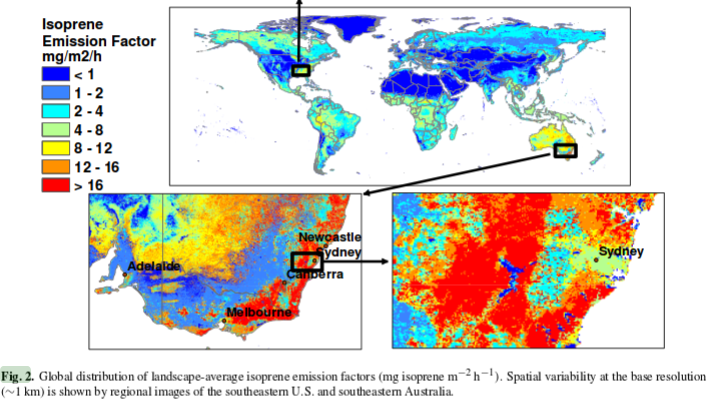
\includegraphics{Figures/MeganIsoprene1.png}
      \caption{ Part of a figure from \citet{Guenther2006} showing global isoprene emission factors. }
      \label{ch1:fig:meganisoprene}
    \end{figure}
    
  \subsection{Isoprene From HCHO}

    Formaldehyde formed in the troposphere is mostly due to VOC oxidation. We can model this oxidation process in order to work out how much VOC is present based on the total HCHO. This requires among other things an idea of which VOCs are present and their yeilds of HCHO.
    In the remote troposphere HCHO production is dominated by methane oxidation, while in the continental boundary layer production is normally due to NMVOCs \citep{Abbot2003,Kefauver2014}

    Satellites recording reflected solar spectra use Differential Optical Absorption Spectroscopy (DOAS) to measure various trace gases in the atmosphere, including formaldehyde. Formaldehyde levels in the continental boundary layer are generally dominated by chemical formation due to VOC (largely isoprene) emissions \citep{Kefauver2014}.
    
    Using satellites allows a broad measure of seasonal and interannual variability of HCHO over Australia. These records can be compared with modeled estimates of HCHO and used as a proxy to estimate isoprene emissions.
    This has been done in North America, South America, and Africa, with satellite and aircraft data combined for validation \citep{Millet_2006, Marais_2014}.
    
    TODO: Read and add this list of sources on the hcho to isop process : taken from Wolfe2015
    Early studies utilized linear steady-state relationships (Palmer et al., 2003), while recent computational advances have permitted full inversions that more fully account for transport, multiple sources and varying chemical regimes (Fortems-Cheiney et al., 2012). Such techniques have informed isoprene emission inventories in North America (Abbot et al., 2003; Millet et al., 2008, 2006; Palmer et al., 2006, 2003), South America (Barkley et al., 2013, 2008), Europe (Curciet al., 2010; Dufour et al., 2009), Africa (Marais et al., 2012), Asia (Fu et al., 2007; Stavrakou et al., 2014), and globally (Fortems-Cheiney et al., 2012; Shim et al., 2005; Stavrakou et al., 2009).

    The methodology for calculating VOCs from HCHO is laid out in \citet{Palmer_2003}, and takes into account the expected lifetime and reaction rates of the precursor VOCs and HCHO.
    Assuming HCHO is produced quickly from short-lived intermediates we get
    \begin{eqnarray*}
    VOC_i \overset{k_i}{\rightarrow} Y_i HCHO
    \end{eqnarray*}
    Where $Y_i$ is HCHO yield per C atom (a measure of how much HCHO will form per gram of C from a VOC within a system).
    Then assuming a steady state of atmospheric HCHO ($\Omega$ molecules $cm^{-2}$) produced by oxidation of VOCs (VOC$_i$) and no horizontal transport:
    \begin{eqnarray*}
    \Omega = \frac{1}{k_{HCHO}} \sum_{i} Y_i E_i
    \end{eqnarray*}
    Where i indexes a chemical species, and $E_i$ is emission fluxes ( C atoms $cm^{-2}s^{-1}$).

    Inferring the VOC emissions then requires estimates of the HCHO yield (Y$_i$) which can be attained via modelling as layed out in \citet{Millet_2006}.

    During low NO$_X$ conditions, the precursor HCHO has a longer lifetime (days).
    This allows horizontal transport to occur and complicates the algorithms.
    Horizontal transport 'smears' the HCHO signal so that source location would need to be calculated using windspeeds and loss rates.
    For conditions where VOCs have a lifetime of days determining the major HCHO contributors requires a complex inversion to map HCHO columns to VOC emissions.

    In high NOx environments where HCHO has a lifetime on the order of 30 minutes, it can be used to map isoprene emissions with spatial resolution from 10-100 kms.
    This can be determined using the calculations from (TODO: cite and formula for spatial resolution)

  \subsection{Measurements}
  
    There are relatively few measurements of isoprene in the southern hemisphere, including MUMBA(TODO CITE), other campaigns?, and very recently that girl from Macquarie University with an instrument in the daintree rainforest(TODO CITE, DESCRIBE?).
    Since 1997, when GOME first measured HCHO over Asia (TODO cite thomas 1998), satellites have been able to provide a total column measurement of one of the primary products of isoprene.
  
  \subsection{Estimates}
    There are two commonly used ways of estimating isoprene emissions, top-down or bottom-up.
    Bottom-up emission estimates generally model the flora and events which emit isoprene, like Eucalypts, factories, fires, etc.
    Understanding how much isoprene is emitted, when and by what is more complicated than it sounds, and since little data exists with which to verify these bottom-up emission inventories they are hard to verify on a large scale.
    Top-down estimates look at how much of a chemical is in the atmosphere and try to work out how much isoprene was emitted. Generally this is done by looking at atmospheric HCHO enhancement, which can be largely attributed to isoprene emissions.
  
  \subsection{Radiative Forcing}

  
%----------------------------------------------------------------------------------------
%	HCHO Section
%----------------------------------------------------------------------------------------
\section{Formaldehyde}
\label{ch1:sec:formaldehyde}
  
  \subsection{Structure}
  TODO: image and description
  
  \subsection{Sources and sinks}
    
    
  \subsection{Measurements}
    There are a few ways to measure HCHO, including FTIR and MAX-DOAS. As a trace gas HCHO interferes with light over a few wavelength bands, which allows instruments to detect concentrations along a path between a sensor and a known light source like a lamp or the sun.
  
%----------------------------------------------------------------------------------------
%	SECTION 5
%----------------------------------------------------------------------------------------
\section{Dust}
\label{ch1:sec:dust}

  Australia is the greatest source of dust in the southern hemisphere producing around 120~Tg yr$^{-1}$ \citep{Li_2008}, however model validation and analysis over Australia is relatively scarce with more focus applied to the northern hemisphere \citep{Duncan_Fairlie_2007,Ridley_2013}.
  Atmospheric dust has many direct effects including reduced surface insolation, mineral transfer to remote ocean regions, and health degradation in populated areas \citep{Shao_2007}.
  Direct and indirect effects of dust have many implications which are not fully understood, with many models still struggling to explain the atmospheric cycling of dust at larger scales \citep{Rotstayn_2011}.

  Australian dust emissions involve various weather conditions, convolving the ENSO cycle with flooding, droughts, and winds.
  Rivers and rain build up the particulate matter in many areas, these are referred to as fluvial deposits.
  Fluvial deposits in the Eyre basin increase the dust base load, which will only have mobility during suitable dry weather conditions.
  These deposits are saltated (loosened from the surface) and transported by strong winds\citep{Zender2003}.

  Synoptic scale measurements of dust concentrations in Australia are made by the Bureau of Meteorology (BOM) and can be used to estimate dust transport caused by large storms. 
  Single storms have been estimated to move up to 2.5 Tg of dust off shore in a single day.
  Yearly dust emissions in Australia are somewhere between 10 and 110 Tg yr$^{-1}$.
  These estimates exemplify the large variability in Australian annual dust transport.

  Dust plays a large role in the oceanic carbon cycle, as dust is a major source of oceanic iron (Fe) deposition.
  Some regions in the ocean are high in nutrients, but low in chlorophyll (HNLC), due to a lack of Fe.
  Oceanic carbon cycling is a complex system in which Fe is a limiting factor, required by plankton in order to fix atmospheric nitrogen into a more bioavailable form such as ammonia.
  Atmospheric deposition into the oceans is a very poorly constrained variable in global models \citep{Grand2015}.
  Model estimates of trace element oceanic deposition are required to quantify the atmospheric impact due to a dearth of in situ measurements in remote open ocean regions.

  Measurements of dissolved iron (DFe) at very low concentrations like those found in surface ocean waters are very easily contaminated, which has contributed the the fragmentary and scarce nature of DFe ocean data sets \citep{Rijkenberg_2014}.
  Recent analysis of the US Climate Variability and Predictability (CLIVAR)-CO$_{2}$ Repeat Hydrography Program predicted total deposition flux with uncertainty at a factor of 3.5 \citep{Grand2015}.
  Some headway has been made with the recent GEOTRACES program which has several transects of the major oceans and measures trace elements over multiple depths including Al, Ba, Cu, Cd, Fe, Mn, Ni, Pb, and Zn.
    
  Total iron (TFe) emissions from dust and combustion sources are estimated (by average of several global models) at approximately 35~Tg yr$^{-1}$ and 2 Tg yr$^{-1}$ respectively. A two fold increase in Fe dissolution may have occurred since 1850 due to increased anthropogenic emissions and atmospheric acidity.
  This increase may revert by 2100 due to the affects of emission regulations \citep{Myriokefalitakis_2015}.
  Dust, TFe and DFe have strong temporally and spatial variability, with changes having most impact upon HnLC regions.

  Another environmental impact of dust is its contribution to fine particulate matter in the atmosphere.
  Several studies have shown that long term exposure to fine particulate matter (PM2.5) increases mortality. 
  Estimates of yearly premature deaths related to PM2.5 are $\sim$ 2-3 million \citep{Hoek_2013, Krewski_2009, Silva_2013, Lelieveld_2015}.   
  These estimates are made using global atmospheric models or model ensembles to quantify population exposure before applying epidemiological models to estimate the increased death rates.
  The main source of uncertainty in premature death rates arises from the difference and uncertainties between and within the atmospheric models.

  Dust affects global climate change through direct radiative forcing.
  Uncertainties in the atmospheric dust concentrations make accurate determination of radiative forcing from other sources more difficult \citep{IPCC_2013_chap8}.


%----------------------------------------------------------------------------------------
%	SECTION 6
%----------------------------------------------------------------------------------------
\section{Models}
\label{ch1:sec:models}

  \subsection{Chemical Transport Models}
  
    Chemical Transport Models (CTMs) simulate production, loss, and transport of chemical species.
    This is generally calculated using one or both of the Eulerian (box) or Lagrangian (puff) frames of reference.
    CTMs normally solve the continuity equations simultaneously with chemical production and loss for chemicals under inspection. 
    The continuity equations describe transport of a conserved quantity such as mass, which, solved together with production and loss of a chemical forms the basis for a CTM.
    This basis enables a record of the chemical densities and transport over time as a model runs.
    The general continuity equation links a quantity of a substance (q) to the field in which it flows and can be described by the formula:
    \begin{eqnarray*}
	\frac{\partial \rho}{\partial t} + \nabla \cdot j &=& \sigma 
    \end{eqnarray*}
    where $\rho$ is density of q in the field, t is time, $\nabla$ is divergence, j is the flux (the amount of q per unit area per unit time entering or leaving the field), and $\sigma$ is the generation of q per unit volume per unit time.
    Note that $\sigma$ can be positive or negative due to sources and sinks.

    The type of model best suited to modelling the entire earth uses the Eulerian frame of reference, where the atmosphere is broken up into 3-D boxes with densities and transport calculated and stored for arbitrary sequential steps in time at each location.
    The mass balance equation must be satisfied in any realistic long term box model and is as follows: 
    \begin{eqnarray*}
	\frac{dm}{dt} &=& \sum{sources}-\sum{sinks} \\
	&=& F_{in} + E + P - F_{out} - L - D 
    \end{eqnarray*}
    where m is mass of a chemical, E and D are emission and deposition, P and L are production and loss, and F is chemical transport in and out, as shown in figure \ref{ch1:fig:boxmodel}.
    Many chemical species interact with each other through production and loss. 
    Any large chemical model will solve this mass balance equation over highly coupled arrays of partial differential equations which can be complex and time consuming.

      
    In many CTMs the isoprene emissions are calculated elsewhere with their own models (EG: \citet{Guenther2006}). These estimates can then be used as boundary conditions. Trace gases with short lifetimes and complex chemistry such as isoprene are often hard to measure which makes verifying model estimates difficult.

    \begin{figure}
      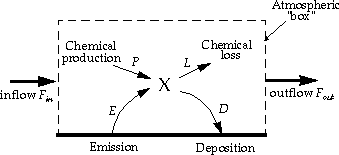
\includegraphics{Figures/boxmodel.png}
      \caption{ Standard box model parameters, image taken from \citet{Jacob_1999_book}. }
      \label{ch1:fig:boxmodel}
    \end{figure}

    
  \subsection{GEOS-Chem}
  
    GEOS-Chem is a well supported global, Eulerian CTM with a state of the science chemical mechanism, with transport driven by meteorological input from the Goddard Earth Observing System (GEOS) of the NASA Global Modeling and Assimilation Office (GMAO).
    GEOS-Chem simulates more than 100 chemical species from the earth's surface up to the edge of space (0.01 hPa) and can be used in combination with remote and in-situ sensing data to give a verifiable estimate of atmospheric gases and aerosols.
    It was developed, and is maintained, by Harvard University staff as well as users and researchers worldwide. 
    Several driving meteorological fields exist with different resolutions, the finest at 0.25 by 0.3125$^\circ$ horizontally at 5 minute time steps with 72 vertical levels.

    Combining satellite data with model outcomes provides a platform for the understanding of natural processes to be tested now and into the future over Australia and anywhere with few in-situ measurements.
    Due to the low availability of in-situ data covering most of the Australian continent, a combination of the models with satellite data may provide improved understanding of emissions from Australian landscapes.
    Improved emissions estimates will in turn improve the accuracy of CTMs, providing better predictions of atmospheric composition and its response to ongoing environmental change.

%----------------------------------------------------------------------------------------
%	SECTION 7
%----------------------------------------------------------------------------------------
\section{Satellites}
\label{ch1:sec:satellites}

  \subsection{Useful satellites}
    Several satellites provide long term trace gas observations with near complete global coverage, including the ERS-2 launched in April 1995 which houses the GOME ultraviolet and visible (UV-Vis) spectrometer, the AURA launched in July 2004 which houses the OMI UV-Vis spectrometer, the MetOp-A and B launched in October 2006 and September 2012 respectively both housing a GOME-2 UV-Vis spectrometer.
    These satellites are on Low Earth Orbit (LEO) trajectories and overpass any area up to once per day. 
    They record near nadir (nearly vertical) reflected spectra between around 250-700~nm split into spectral components at around $0.3$~nm in order to calculate trace gases including O$_3$, NO$_2$, and HCHO.
    An example of a spectrum retrieved from the GOME-2 instrument is given in figure \ref{ch1:fig:gomeproducts}.

    \begin{figure}
      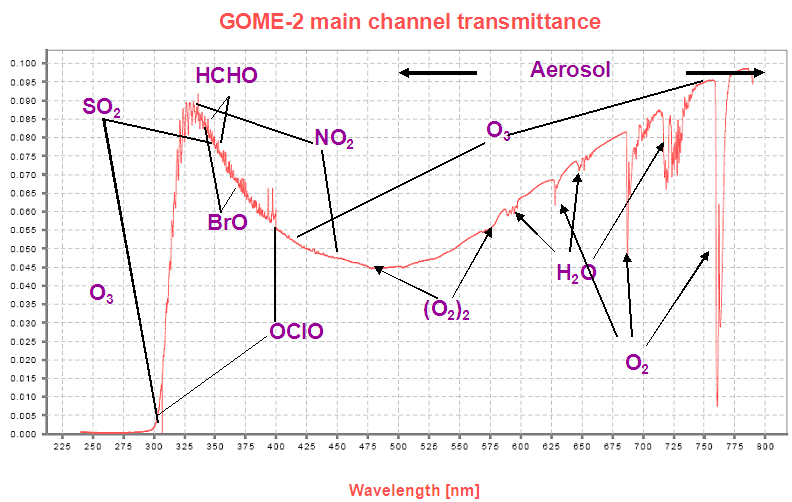
\includegraphics[width=\textwidth]{Figures/GOME_SPECTRUM.jpg}
      \caption{An example spectrum showing interferences used for species concentration measurements by GOME-2. Image by EUMETSAT and ESA \citep{GOME2Image}.}
      \label{ch1:fig:gomeproducts}
    \end{figure}

    
    Formaldehyde (HCHO) is often used as a proxy to estimate isoprene emissions \citep{Marais_2012,bauwens2013satellite}.
    Satellites can use DOAS techniques with radiative transfer calculations on solar radiation absorption spectra to measure column HCHO (eg: \citet{Leue_2001}).
    Several public data servers are available which include products from the satellites just mentioned, including NASA's Mirador (http://mirador.gsfc.nasa.gov/) and the Belgian Institute for Space Aeronomy (IASB-BIRA) Aeronomie site (http://h2co.aeronomie.be/).

    Instruments including MODIS on board the AQUA and TERRA satellites are able to determine aerosol optical depth (AOD), a measure of atmospheric scatter and absorbance. 
    An AOD of under 0.05 indicates a clear sky, while values of 1 or greater indicate increasingly hazy conditions.
    This is an important atmospheric property allowing us to track dust storms and pollution events as well as determine where measurements from other instruments may be compromised by high AOD.
    Satellite measured AOD requires validation by more accurate ground based instruments like those of AERONET which uses more than 200 sun photometers scattered globally. 
  
  \subsection{Comparisons with Models}
  
    DOAS methods can be heavily influenced by the initial estimates of a trace gas profile (the a priori) which is often produced by modelling, so when comparing models of these trace gases to satellite measurements extra care needs to be taken to avoid introducing bias from unrealistic a priori assumptions.
    A way to remove these a priori influences in order to compare models and satellites is through the satellite's averaging kernal, which is a measure of the sensitivity of the instrument to the trace gas's radiance at various heights multiplied by the sensitivity of the DOAS technique's forward radiative transfer model (RTM) to the amount of trace gas at various heights near the a priori \citep{Eskes_2003}.
  
  \subsection{DOAS}
    TODO: some of this is repeated in isoprene chapter satellite section.
    
    The DOAS technique uses solar radiation absorption spectra to measure trace gases through paths of light.
    The RTM used in DOAS techniques is based on Beer's law relating the attenuation of light to the properties of the medium it travels through.
    Beer's law states that $ T = I/I_0 = e^{-\tau} $ with T being transmittance, $\tau$ being optical depth, and I, I$_0$ being radiant flux received at instrument and emitted at source respectively.
    Using 
    $ \tau_i = \int \rho_i \beta_i ds $ gives us:
    $$ I = I_0 \exp {\left( \Sigma_i \int \rho_i \beta_i ds \right) } $$
    Where i represents a chemical species index, $\rho$ is a species density(molecules per cm$^3$), $\beta$ is the scattering and absorption cross section area (cm$^2$), and the integral over ds represents integration over the path from light source to instrument.
    The forward RTM used for satellite data products also involves functions representing extinction from Mie and Rayleigh scattering, and the efficiency of these on intensities from the trace gas under inspection, as well as accounting for various atmospheric parameters which may or may not be estimated (e.g. albedo).
    
    To convert the trace gas profile from a reflected solar radiance column (slanted along the light path) into a purely vertical column requires calculations of an air mass factor (AMF).
    In satellite data, the AMF is typically a scalar value for each horizontal grid point which will equal the ratio of the total vertical column density to the total slant column density. This value should also account for instrument sensitivities to various wavelengths at various altitudes, and is unique for each trace gas under consideration.
  
%\include{Chapters/Chapter2} 
%\include{Chapters/Chapter3}
%\include{Chapters/Chapter4} 
%\include{Chapters/Chapter5} 

%----------------------------------------------------------------------------------------
%	THESIS CONTENT - APPENDICES
%----------------------------------------------------------------------------------------

\appendix % Cue to tell LaTeX that the following "chapters" are Appendices

% Include the appendices of the thesis as separate files from the Appendices folder
% Uncomment the lines as you write the Appendices

% Appendix A

\chapter{Appendix A} % Main appendix title
\label{app_a}

% figures.tex created in python in appendices folder
%\section{Melbourne}
  \includegraphics[width=\textwidth]{../OzoneWork/Images/AIRS/Melbourne/2007-01-12.png}
  \includegraphics[width=\textwidth]{../OzoneWork/Images/AIRS/Melbourne/2011-08-24.png}
  \includegraphics[width=\textwidth]{../OzoneWork/Images/AIRS/Melbourne/2012-10-30.png}
  \includegraphics[width=\textwidth]{../OzoneWork/Images/AIRS/Melbourne/2011-03-09.png}
  \includegraphics[width=\textwidth]{../OzoneWork/Images/AIRS/Melbourne/2013-01-16.png}
  \includegraphics[width=\textwidth]{../OzoneWork/Images/AIRS/Melbourne/2007-04-20.png}
  \includegraphics[width=\textwidth]{../OzoneWork/Images/AIRS/Melbourne/2005-11-08.png}
  \includegraphics[width=\textwidth]{../OzoneWork/Images/AIRS/Melbourne/2011-05-11.png}
  \includegraphics[width=\textwidth]{../OzoneWork/Images/AIRS/Melbourne/2006-02-03.png}
  \includegraphics[width=\textwidth]{../OzoneWork/Images/AIRS/Melbourne/2008-02-21.png}
  \includegraphics[width=\textwidth]{../OzoneWork/Images/AIRS/Melbourne/2009-01-07.png}
  \includegraphics[width=\textwidth]{../OzoneWork/Images/AIRS/Melbourne/2012-02-23.png}
  \includegraphics[width=\textwidth]{../OzoneWork/Images/AIRS/Melbourne/2011-02-23.png}
  \includegraphics[width=\textwidth]{../OzoneWork/Images/AIRS/Melbourne/2013-01-04.png}
  \includegraphics[width=\textwidth]{../OzoneWork/Images/AIRS/Melbourne/2007-10-17.png}
  \includegraphics[width=\textwidth]{../OzoneWork/Images/AIRS/Melbourne/2013-01-11.png}
  \includegraphics[width=\textwidth]{../OzoneWork/Images/AIRS/Melbourne/2011-03-16.png}
  \includegraphics[width=\textwidth]{../OzoneWork/Images/AIRS/Melbourne/2006-10-16.png}
  \includegraphics[width=\textwidth]{../OzoneWork/Images/AIRS/Melbourne/2009-01-13.png}
  \includegraphics[width=\textwidth]{../OzoneWork/Images/AIRS/Melbourne/2008-11-26.png}
  \includegraphics[width=\textwidth]{../OzoneWork/Images/AIRS/Melbourne/2013-03-20.png}
  \includegraphics[width=\textwidth]{../OzoneWork/Images/AIRS/Melbourne/2007-04-13.png}
  \includegraphics[width=\textwidth]{../OzoneWork/Images/AIRS/Melbourne/2011-07-13.png}
  \includegraphics[width=\textwidth]{../OzoneWork/Images/AIRS/Melbourne/2008-12-03.png}
  \includegraphics[width=\textwidth]{../OzoneWork/Images/AIRS/Melbourne/2009-09-23.png}
  \includegraphics[width=\textwidth]{../OzoneWork/Images/AIRS/Melbourne/2010-10-27.png}
  \includegraphics[width=\textwidth]{../OzoneWork/Images/AIRS/Melbourne/2011-02-17.png}
  \includegraphics[width=\textwidth]{../OzoneWork/Images/AIRS/Melbourne/2009-09-16.png}
  \includegraphics[width=\textwidth]{../OzoneWork/Images/AIRS/Melbourne/2010-09-02.png}
  \includegraphics[width=\textwidth]{../OzoneWork/Images/AIRS/Melbourne/2012-03-14.png}
  \includegraphics[width=\textwidth]{../OzoneWork/Images/AIRS/Melbourne/2013-05-01.png}
  \includegraphics[width=\textwidth]{../OzoneWork/Images/AIRS/Melbourne/2007-01-04.png}
  \includegraphics[width=\textwidth]{../OzoneWork/Images/AIRS/Melbourne/2010-07-07.png}
  \includegraphics[width=\textwidth]{../OzoneWork/Images/AIRS/Melbourne/2006-02-17.png}
  \includegraphics[width=\textwidth]{../OzoneWork/Images/AIRS/Melbourne/2012-10-03.png}
  \includegraphics[width=\textwidth]{../OzoneWork/Images/AIRS/Melbourne/2005-01-13.png}
  \includegraphics[width=\textwidth]{../OzoneWork/Images/AIRS/Melbourne/2011-12-07.png}
  \includegraphics[width=\textwidth]{../OzoneWork/Images/AIRS/Melbourne/2008-07-09.png}
  \includegraphics[width=\textwidth]{../OzoneWork/Images/AIRS/Melbourne/2004-10-07.png}
  \includegraphics[width=\textwidth]{../OzoneWork/Images/AIRS/Melbourne/2010-03-10.png}
  \includegraphics[width=\textwidth]{../OzoneWork/Images/AIRS/Melbourne/2010-06-02.png}
  \includegraphics[width=\textwidth]{../OzoneWork/Images/AIRS/Melbourne/2006-08-09.png}
  \includegraphics[width=\textwidth]{../OzoneWork/Images/AIRS/Melbourne/2011-02-15.png}
  \includegraphics[width=\textwidth]{../OzoneWork/Images/AIRS/Melbourne/2011-10-25.png}
  \includegraphics[width=\textwidth]{../OzoneWork/Images/AIRS/Melbourne/2008-12-12.png}
  \includegraphics[width=\textwidth]{../OzoneWork/Images/AIRS/Melbourne/2010-01-28.png}
  \includegraphics[width=\textwidth]{../OzoneWork/Images/AIRS/Melbourne/2011-04-20.png}
  \includegraphics[width=\textwidth]{../OzoneWork/Images/AIRS/Melbourne/2005-10-26.png}
  \includegraphics[width=\textwidth]{../OzoneWork/Images/AIRS/Melbourne/2008-01-18.png}
  \includegraphics[width=\textwidth]{../OzoneWork/Images/AIRS/Melbourne/2009-01-30.png}
  \includegraphics[width=\textwidth]{../OzoneWork/Images/AIRS/Melbourne/2009-12-23.png}
  \includegraphics[width=\textwidth]{../OzoneWork/Images/AIRS/Melbourne/2013-02-01.png}
  \includegraphics[width=\textwidth]{../OzoneWork/Images/AIRS/Melbourne/2006-03-02.png}
  \includegraphics[width=\textwidth]{../OzoneWork/Images/AIRS/Melbourne/2010-01-13.png}
  \includegraphics[width=\textwidth]{../OzoneWork/Images/AIRS/Melbourne/2006-07-20.png}
  \includegraphics[width=\textwidth]{../OzoneWork/Images/AIRS/Melbourne/2004-01-08.png}
  \includegraphics[width=\textwidth]{../OzoneWork/Images/AIRS/Melbourne/2005-04-14.png}
  \includegraphics[width=\textwidth]{../OzoneWork/Images/AIRS/Melbourne/2005-11-03.png}
  \includegraphics[width=\textwidth]{../OzoneWork/Images/AIRS/Melbourne/2010-02-03.png}
  \includegraphics[width=\textwidth]{../OzoneWork/Images/AIRS/Melbourne/2007-03-15.png}
  \includegraphics[width=\textwidth]{../OzoneWork/Images/AIRS/Melbourne/2011-02-09.png}
  \includegraphics[width=\textwidth]{../OzoneWork/Images/AIRS/Melbourne/2009-07-21.png}
  \includegraphics[width=\textwidth]{../OzoneWork/Images/AIRS/Melbourne/2010-11-03.png}
  \includegraphics[width=\textwidth]{../OzoneWork/Images/AIRS/Melbourne/2009-09-02.png}
  \includegraphics[width=\textwidth]{../OzoneWork/Images/AIRS/Melbourne/2010-04-07.png}
  \includegraphics[width=\textwidth]{../OzoneWork/Images/AIRS/Melbourne/2005-11-17.png}
  \includegraphics[width=\textwidth]{../OzoneWork/Images/AIRS/Melbourne/2010-03-04.png}
  \includegraphics[width=\textwidth]{../OzoneWork/Images/AIRS/Melbourne/2012-12-21.png}
  \includegraphics[width=\textwidth]{../OzoneWork/Images/AIRS/Melbourne/2004-02-02.png}
  \includegraphics[width=\textwidth]{../OzoneWork/Images/AIRS/Melbourne/2007-03-28.png}
  \includegraphics[width=\textwidth]{../OzoneWork/Images/AIRS/Melbourne/2013-10-04.png}
  \includegraphics[width=\textwidth]{../OzoneWork/Images/AIRS/Melbourne/2007-10-31.png}
  \includegraphics[width=\textwidth]{../OzoneWork/Images/AIRS/Melbourne/2007-03-21.png}
\section{Macquarie}
  \includegraphics[width=\textwidth]{../OzoneWork/Images/AIRS/Macquarie/2009-02-18.png}
  \includegraphics[width=\textwidth]{../OzoneWork/Images/AIRS/Macquarie/2004-02-04.png}
  \includegraphics[width=\textwidth]{../OzoneWork/Images/AIRS/Macquarie/2011-05-11.png}
  \includegraphics[width=\textwidth]{../OzoneWork/Images/AIRS/Macquarie/2004-05-19.png}
  \includegraphics[width=\textwidth]{../OzoneWork/Images/AIRS/Macquarie/2005-08-25.png}
  \includegraphics[width=\textwidth]{../OzoneWork/Images/AIRS/Macquarie/2010-02-10.png}
  \includegraphics[width=\textwidth]{../OzoneWork/Images/AIRS/Macquarie/2009-01-21.png}
  \includegraphics[width=\textwidth]{../OzoneWork/Images/AIRS/Macquarie/2005-01-12.png}
  \includegraphics[width=\textwidth]{../OzoneWork/Images/AIRS/Macquarie/2009-01-07.png}
  \includegraphics[width=\textwidth]{../OzoneWork/Images/AIRS/Macquarie/2010-02-24.png}
  \includegraphics[width=\textwidth]{../OzoneWork/Images/AIRS/Macquarie/2010-01-27.png}
  \includegraphics[width=\textwidth]{../OzoneWork/Images/AIRS/Macquarie/2008-03-21.png}
  \includegraphics[width=\textwidth]{../OzoneWork/Images/AIRS/Macquarie/2005-01-19.png}
  \includegraphics[width=\textwidth]{../OzoneWork/Images/AIRS/Macquarie/2006-10-12.png}
  \includegraphics[width=\textwidth]{../OzoneWork/Images/AIRS/Macquarie/2012-12-19.png}
  \includegraphics[width=\textwidth]{../OzoneWork/Images/AIRS/Macquarie/2007-01-17.png}
  \includegraphics[width=\textwidth]{../OzoneWork/Images/AIRS/Macquarie/2004-03-10.png}
  \includegraphics[width=\textwidth]{../OzoneWork/Images/AIRS/Macquarie/2008-06-04.png}
  \includegraphics[width=\textwidth]{../OzoneWork/Images/AIRS/Macquarie/2004-06-09.png}
  \includegraphics[width=\textwidth]{../OzoneWork/Images/AIRS/Macquarie/2010-03-31.png}
  \includegraphics[width=\textwidth]{../OzoneWork/Images/AIRS/Macquarie/2009-01-14.png}
  \includegraphics[width=\textwidth]{../OzoneWork/Images/AIRS/Macquarie/2008-10-22.png}
  \includegraphics[width=\textwidth]{../OzoneWork/Images/AIRS/Macquarie/2004-03-05.png}
  \includegraphics[width=\textwidth]{../OzoneWork/Images/AIRS/Macquarie/2009-12-09.png}
  \includegraphics[width=\textwidth]{../OzoneWork/Images/AIRS/Macquarie/2005-12-21.png}
  \includegraphics[width=\textwidth]{../OzoneWork/Images/AIRS/Macquarie/2011-04-06.png}
  \includegraphics[width=\textwidth]{../OzoneWork/Images/AIRS/Macquarie/2009-09-09.png}
  \includegraphics[width=\textwidth]{../OzoneWork/Images/AIRS/Macquarie/2004-10-20.png}
  \includegraphics[width=\textwidth]{../OzoneWork/Images/AIRS/Macquarie/2011-12-07.png}
  \includegraphics[width=\textwidth]{../OzoneWork/Images/AIRS/Macquarie/2009-08-26.png}
  \includegraphics[width=\textwidth]{../OzoneWork/Images/AIRS/Macquarie/2011-02-16.png}
  \includegraphics[width=\textwidth]{../OzoneWork/Images/AIRS/Macquarie/2010-03-10.png}
  \includegraphics[width=\textwidth]{../OzoneWork/Images/AIRS/Macquarie/2011-01-19.png}
  \includegraphics[width=\textwidth]{../OzoneWork/Images/AIRS/Macquarie/2011-09-21.png}
  \includegraphics[width=\textwidth]{../OzoneWork/Images/AIRS/Macquarie/2009-06-24.png}
  \includegraphics[width=\textwidth]{../OzoneWork/Images/AIRS/Macquarie/2005-03-28.png}
  \includegraphics[width=\textwidth]{../OzoneWork/Images/AIRS/Macquarie/2009-12-23.png}
  \includegraphics[width=\textwidth]{../OzoneWork/Images/AIRS/Macquarie/2012-03-29.png}
  \includegraphics[width=\textwidth]{../OzoneWork/Images/AIRS/Macquarie/2005-10-19.png}
  \includegraphics[width=\textwidth]{../OzoneWork/Images/AIRS/Macquarie/2008-02-13.png}
  \includegraphics[width=\textwidth]{../OzoneWork/Images/AIRS/Macquarie/2006-02-01.png}
  \includegraphics[width=\textwidth]{../OzoneWork/Images/AIRS/Macquarie/2009-03-18.png}
  \includegraphics[width=\textwidth]{../OzoneWork/Images/AIRS/Macquarie/2012-08-09.png}
  \includegraphics[width=\textwidth]{../OzoneWork/Images/AIRS/Macquarie/2011-02-03.png}
  \includegraphics[width=\textwidth]{../OzoneWork/Images/AIRS/Macquarie/2004-02-25.png}
  \includegraphics[width=\textwidth]{../OzoneWork/Images/AIRS/Macquarie/2012-09-26.png}
  \includegraphics[width=\textwidth]{../OzoneWork/Images/AIRS/Macquarie/2006-11-08.png}
  \includegraphics[width=\textwidth]{../OzoneWork/Images/AIRS/Macquarie/2012-08-16.png}
  \includegraphics[width=\textwidth]{../OzoneWork/Images/AIRS/Macquarie/2007-03-14.png}
  \includegraphics[width=\textwidth]{../OzoneWork/Images/AIRS/Macquarie/2007-03-08.png}
\section{Davis}
  \includegraphics[width=\textwidth]{../OzoneWork/Images/AIRS/Davis/2012-11-24.png}
  \includegraphics[width=\textwidth]{../OzoneWork/Images/AIRS/Davis/2011-03-09.png}
  \includegraphics[width=\textwidth]{../OzoneWork/Images/AIRS/Davis/2011-12-14.png}
  \includegraphics[width=\textwidth]{../OzoneWork/Images/AIRS/Davis/2011-01-12.png}
  \includegraphics[width=\textwidth]{../OzoneWork/Images/AIRS/Davis/2011-04-13.png}
  \includegraphics[width=\textwidth]{../OzoneWork/Images/AIRS/Davis/2012-12-03.png}
  \includegraphics[width=\textwidth]{../OzoneWork/Images/AIRS/Davis/2011-06-29.png}
  \includegraphics[width=\textwidth]{../OzoneWork/Images/AIRS/Davis/2007-01-15.png}
  \includegraphics[width=\textwidth]{../OzoneWork/Images/AIRS/Davis/2012-03-21.png}
  \includegraphics[width=\textwidth]{../OzoneWork/Images/AIRS/Davis/2008-06-04.png}
  \includegraphics[width=\textwidth]{../OzoneWork/Images/AIRS/Davis/2012-10-13.png}
  \includegraphics[width=\textwidth]{../OzoneWork/Images/AIRS/Davis/2008-06-11.png}
  \includegraphics[width=\textwidth]{../OzoneWork/Images/AIRS/Davis/2008-10-22.png}
  \includegraphics[width=\textwidth]{../OzoneWork/Images/AIRS/Davis/2009-09-23.png}
  \includegraphics[width=\textwidth]{../OzoneWork/Images/AIRS/Davis/2010-09-23.png}
  \includegraphics[width=\textwidth]{../OzoneWork/Images/AIRS/Davis/2009-07-01.png}
  \includegraphics[width=\textwidth]{../OzoneWork/Images/AIRS/Davis/2012-07-19.png}
  \includegraphics[width=\textwidth]{../OzoneWork/Images/AIRS/Davis/2006-09-30.png}
  \includegraphics[width=\textwidth]{../OzoneWork/Images/AIRS/Davis/2010-12-10.png}
  \includegraphics[width=\textwidth]{../OzoneWork/Images/AIRS/Davis/2011-03-04.png}
  \includegraphics[width=\textwidth]{../OzoneWork/Images/AIRS/Davis/2006-09-22.png}
  \includegraphics[width=\textwidth]{../OzoneWork/Images/AIRS/Davis/2012-02-15.png}
  \includegraphics[width=\textwidth]{../OzoneWork/Images/AIRS/Davis/2013-10-23.png}
  \includegraphics[width=\textwidth]{../OzoneWork/Images/AIRS/Davis/2012-04-12.png}
  \includegraphics[width=\textwidth]{../OzoneWork/Images/AIRS/Davis/2009-06-24.png}
  \includegraphics[width=\textwidth]{../OzoneWork/Images/AIRS/Davis/2007-08-11.png}
  \includegraphics[width=\textwidth]{../OzoneWork/Images/AIRS/Davis/2007-12-11.png}
  \includegraphics[width=\textwidth]{../OzoneWork/Images/AIRS/Davis/2009-11-21.png}
  \includegraphics[width=\textwidth]{../OzoneWork/Images/AIRS/Davis/2007-04-17.png}
  \includegraphics[width=\textwidth]{../OzoneWork/Images/AIRS/Davis/2008-03-14.png}
  \includegraphics[width=\textwidth]{../OzoneWork/Images/AIRS/Davis/2006-06-06.png}
  \includegraphics[width=\textwidth]{../OzoneWork/Images/AIRS/Davis/2011-07-20.png}
  \includegraphics[width=\textwidth]{../OzoneWork/Images/AIRS/Davis/2009-10-07.png}
  \includegraphics[width=\textwidth]{../OzoneWork/Images/AIRS/Davis/2012-01-25.png}
  \includegraphics[width=\textwidth]{../OzoneWork/Images/AIRS/Davis/2007-02-16.png}
  \includegraphics[width=\textwidth]{../OzoneWork/Images/AIRS/Davis/2013-08-21.png}

  
\section{Grid Resolution}
% grid created using ctm_grid output -> text created by levels_table.py in extras
\begin{table}
  \begin{tabular}{|l|c|c|}
    \hline
    Level & z(km) & eta 
    \\ \hline
    1 & 0.058483 & 0.99250000 
    \\ \hline
    2 & 0.188515 & 0.97745600 
    \\ \hline
    3 & 0.320427 & 0.96237000 
    \\ \hline
    4 & 0.453892 & 0.94728500 
    \\ \hline
    5 & 0.588963 & 0.93220000 
    \\ \hline
    6 & 0.725697 & 0.91711600 
    \\ \hline
    7 & 0.864132 & 0.90203100 
    \\ \hline
    8 & 1.004320 & 0.88694800 
    \\ \hline
    9 & 1.146330 & 0.87186400 
    \\ \hline
    10 & 1.290220 & 0.85678100 
    \\ \hline
    11 & 1.436040 & 0.84169800 
    \\ \hline
    12 & 1.583870 & 0.82661600 
    \\ \hline
    13 & 1.758950 & 0.80902100 
    \\ \hline
    14 & 1.988400 & 0.78640000 
    \\ \hline
    15 & 2.249380 & 0.76126500 
    \\ \hline
    16 & 2.517070 & 0.73613400 
    \\ \hline
    17 & 2.791920 & 0.71100600 
    \\ \hline
    18 & 3.074460 & 0.68587800 
    \\ \hline
    19 & 3.439220 & 0.65447100 
    \\ \hline
    20 & 3.895550 & 0.61679000 
    \\ \hline
    21 & 4.374520 & 0.57911500 
    \\ \hline
    22 & 4.879030 & 0.54144900 
    \\ \hline
    23 & 5.412570 & 0.50379500 
    \\ \hline
    24 & 5.979530 & 0.46615300 
    \\ \hline
    25 & 6.585330 & 0.42852800 
    \\ \hline
    26 & 7.236820 & 0.39092700 
    \\ \hline
    27 & 7.943070 & 0.35334900 
    \\ \hline
    28 & 8.845840 & 0.30985400 
    \\ \hline
    29 & 9.936460 & 0.26358700 
    \\ \hline
    30 & 11.020800 & 0.22377200 
    \\ \hline
    31 & 12.085500 & 0.19006100 
    \\ \hline
    32 & 13.133500 & 0.16151300 
    \\ \hline
    33 & 14.169600 & 0.13728700 
    \\ \hline
    34 & 15.198200 & 0.11669500 
    \\ \hline
    35 & 16.221700 & 0.09919110 
    \\ \hline
    36 & 17.242600 & 0.08431270 
    \\ \hline
    37 & 18.727200 & 0.06655890 
    \\ \hline
    38 & 20.835700 & 0.04764090 
    \\ \hline
    39 & 23.020500 & 0.03381390 
    \\ \hline
    40 & 25.306800 & 0.02375520 
    \\ \hline
    41 & 28.654300 & 0.01434240 
    \\ \hline
    42 & 34.024400 & 0.00658754 
    \\ \hline
    43 & 40.166100 & 0.00281639 
    \\ \hline
    44 & 47.135400 & 0.00110910 
    \\ \hline
    45 & 54.833600 & 0.00039878 
    \\ \hline
    46 & 63.052800 & 0.00012699 
    \\ \hline
    47 & 72.180100 & 0.00002763 
    \\ \hline
  \end{tabular}
  \caption{The 47 level vertical grid used by GEOS-Chem}
  \label{app_a:tab:gc_47_vgrid}
\end{table}
%\include{Appendices/AppendixB}
%\include{Appendices/AppendixC}

%----------------------------------------------------------------------------------------
%	BIBLIOGRAPHY
%----------------------------------------------------------------------------------------

\printbibliography[heading=bibintoc]

%----------------------------------------------------------------------------------------

\end{document}  
